As Dennard scaling ends, big-data applications such as real-time image processing, graph analytics, and deep learning continue to push the boundaries of performance and energy efficiency requirements for compute system. 
One solution to this challenge is to move compute closer to memory or storage for substantial energy savings of data movement. 
We have developed an innovative Near-Data Computing (NDC) architecture that leverages the dramatic opportunities provided by the new CXL protocol. 
NDC incorporates heterogenous compute elements in the memory/storage subsystem to accelerate various computing tasks near data. 
One of these compute elements is the Streaming Engine (SE).

The SE is a Coarse-Grained Reconfigurable Array (CGRA) that is composed of interconnected compute tiles.  
The compute tiles are interconnected with both a Synchronous Fabric (SF) and an Asynchronous Fabric (AF) as shown in Fig. \ref{fig:se_diagram}.
It also interconnects tile memory, multiplexers, and Single Instruction Multiple Data (SIMD) units within each tile. 
Tiles can be pipelined through SF to form a synchronous data flow (SDF) through Multiply/Shift (MS) unit and an Arithmetic/Logic (AL) SIMD units. 
The Output of the MS unit is connected the one of the two inputs onf the AL unit.
AF connects a tile with all other tiles, dispatch interface (DI), and memory interfaces (MIs).
It bridges SDFs through asynchronous operations, which include SDF initiation, asynchronous data transfer from one SDF to another, system memory accesses, and branching and looping constructs. 
Together, SF and AF allow the tiles to efficiently execute high-level programming language constructs. 
Simulation results of hand-crafted SE kernels have shown orders-of-magnitude better performance per watt on data-intensive applications than existing computing platforms.


Mapping the instructions from the computation graph of a program onto the compute elements of the SE while adhering to architectural constraints is an NP-complete problem with a vast and sparse search space. 
Constraints related to tile memory and synchronous dataflow, use of delays to match timing requirements and more are necessary to ensure correct execution. 
Creating the mappings manually or using brute force algorithms takes time and lots of effort. 
This process also adds assumptions that reduce the search space, trading off optimization possibilities.  

A simple example that demonstrates how a program is mapped to and executed by the SE is shown in Fig. \ref{fig:se_example}.
Mapping the distance calculation function, Eq. \ref{eq:dist} to the SE.

\begin{equation}
    \label{eq:dist}
    D = \sqrt{(x - x_0)^2 +(y - y_0)^2 + (z - z_0)^2}
\end{equation}

To keep this example simple, we ignore the square root part of the equation.
The programmer rewrites the program as a directed Acyclic Graph (DAG) as shown in Fig. \ref{fig:se_example}.

Each operation in Eq. \ref{eq:dist} is an instruction that is mapped to a slot at a tile on the SE.
Each instruction can include both a multiplication and an addition, as shown in Eq. \ref{eq:msal}:

\begin{equation}
    \label{eq:msal}
    MS/AL_{output} = (MS_{in1} \times MS_{in2}) + AL_{in2} 
\end{equation}

Hence, instruction 6 combines the multiplication of $\Delta z^2$ with the addition of the previous result of $(\Delta x^2 + \Delta y^2)$.

\begin{figure}
    \centering
    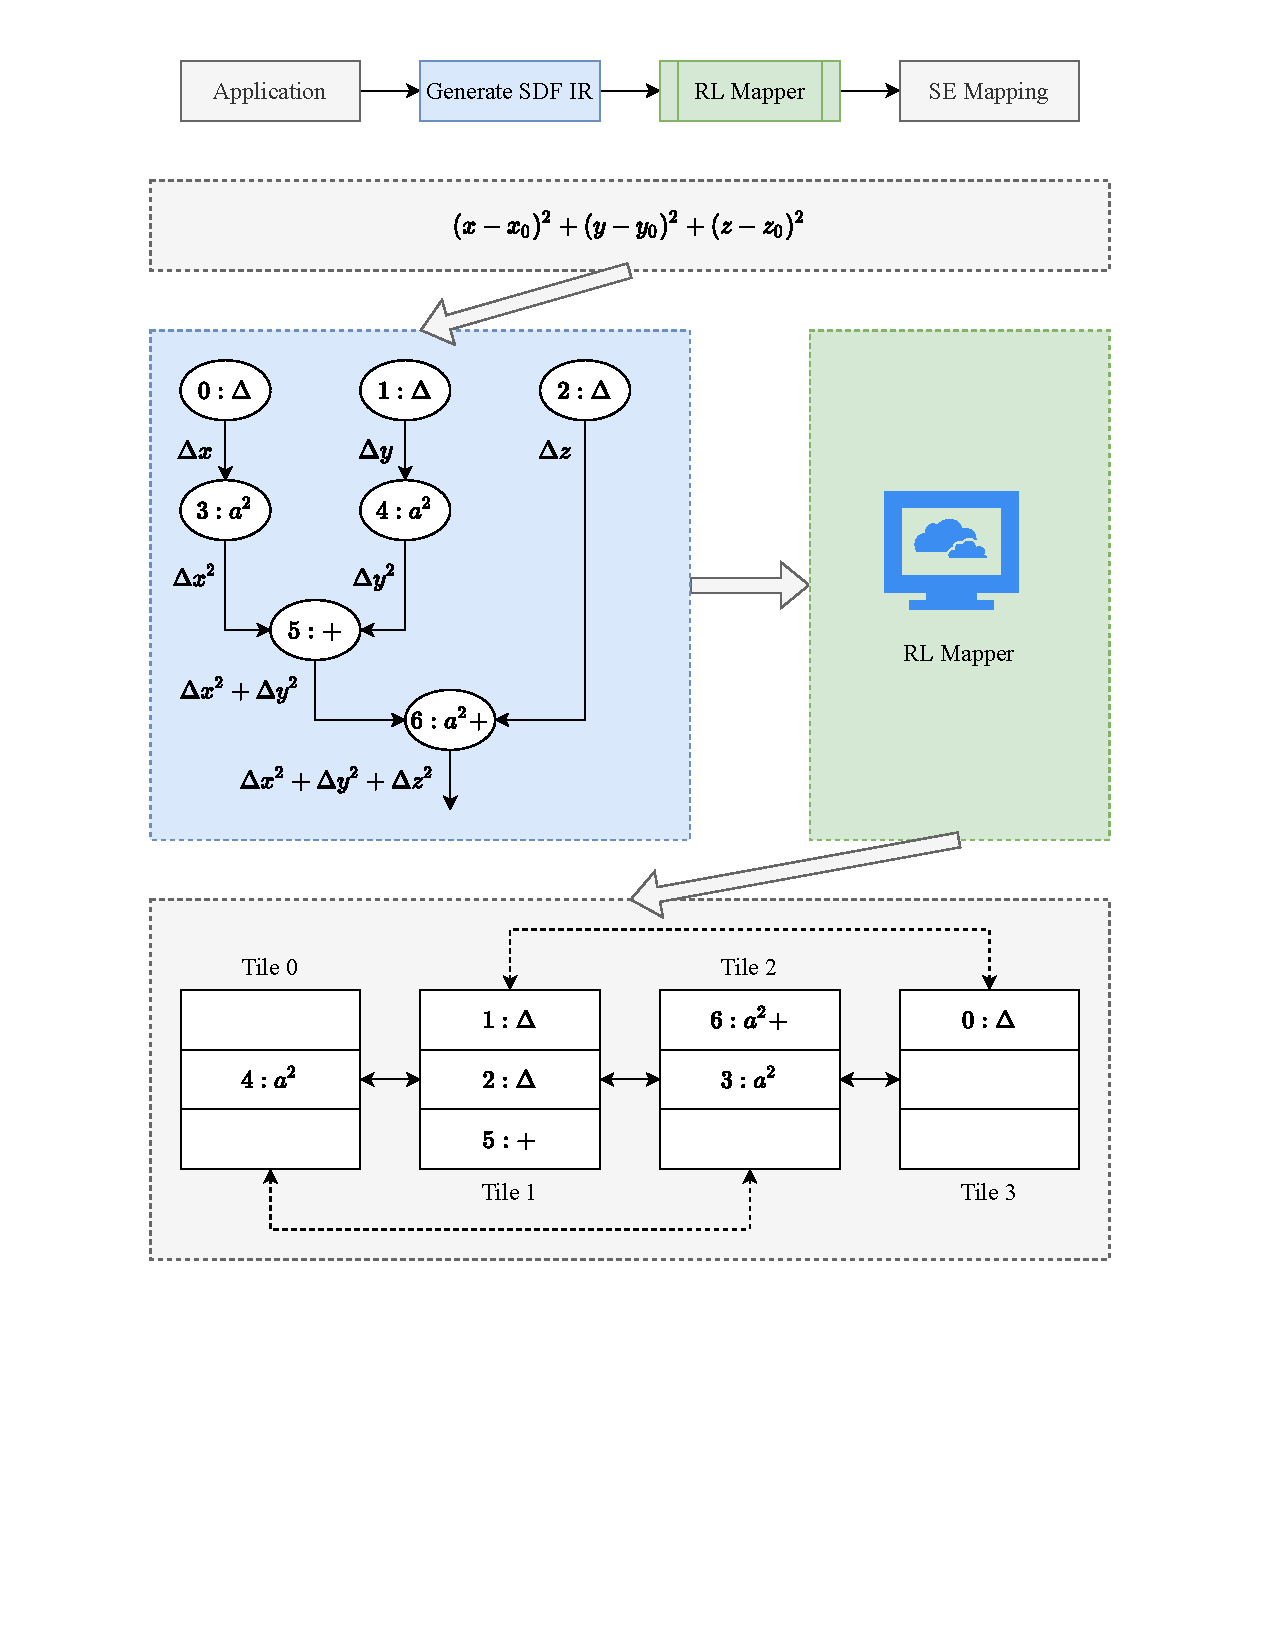
\includegraphics[trim=70 180 70 25, clip, width=\linewidth]{fig/SE_example.pdf}
    \caption{
      Example showing the high-level steps of mapping of distance calculation using the SE device.
      The solid lines connecting the tiles, represent an SF connection with one clock cycle latency.
      The dotted lines connecting the tiles, represent an SF connection with two clock cycles latency.
      The pipeline latency for an instruction is three clock cycles.
      For example, instruction \#0 is scheduled at slot \#0 of tile \#3 and its output is sent to instruction \#3.
      The result of instruction \#0 is ready after three clock cycles, in addition to two clock cycles to move the result to tile \#1, instruction \#3 is correctly scheduled on on slot \#1 of tile \#1.
    }
    \label{fig:se_example}
  \end{figure}


In this work we propose a Deep Reinforcement Learning (RL) method to explore and find optimal mappings in an unsupervised manner. 
Using the Proximal Policy Optimization (PPO) method we train a neural network model to place instructions onto the SE tiles guided by a reward function that models the SE device and its constraints. 
The trained model was able to create valid mappings for the SE by learning about the problem domain. 
By using a learning methodology, we are able to reuse what the neural network learned to obtain mappings for computation graphs that were not seen during training.  

This work is motivated to provide improved tools set that lowers SE usability barrier.
This also assist other tools or programmers in SE mapping creation by providing placement suggestions or tile configuration labels.
The RL mapper performs unsupervised learning and optimization allowing it to search a wide and sparse search space. 
Each operation is an instruction that is mapped to a specific slot on a tile.

This line of research is inspired by recent work that used RL for chip placement.
Our problem requirement of mapping nodes of a computation graph to available compute elements is similar to the problem of placing nodes of a chip netlist on a chip canvas. 

Our main contributions are:
\begin{enumerate}
    \item contribution 1
    \item contribution 2
    \item ... etc.
\end{enumerate}

The rest of this paper is organized as follows: Section \ref{sec:background} provides the necessary background on the SE device architecture.
Section \ref{sec:rlmapper} presents the proposed RL approach for mapping applications to the SE.
Finally, Section \ref{sec:relatedwork} discusses related work and Section \ref{sec:conclusion} provides conclusions and future work.